\documentclass[12pt]{article}
\usepackage{fullpage,enumitem,amsmath,amssymb,graphicx}

\usepackage{lipsum}
\usepackage{multicol}
\usepackage{cite}

\begin{document}

\title{Learning to Walk: A Tale of Jackrabbot's Path-finding Adventures \\
\Large CS231A Winter 2015 Project Proposal}

\date{\today}

\author{
\begin{tabular}{c c c}
Kathy Sun && John Doherty \\
kathysun && doherty1 \\
\end{tabular} }

\maketitle

\section{Introduction}

The Jackrabbot is an autonomous delivery robot designed to share pedestrian walkways. In contrast to autonomous vehicles, this proposes the challenges of interacting safely with humans and bikers in a socially acceptable fashion. The path of the Jackrabbot then becomes nontrivial, as it cannot block pedestrian traffic or scare fellow travelers. The goal of our project is to develop a path-planning algorithm for the Jackrabbot that learns from observing the path-finding behaviors of the humans it will share walkways with. 

Path-finding and obstacle avoidance has been an active area in research since the development of autonomous vehicles.  The Jackrabbot faces the additional challenges of interacting safely with humans and bikers on pedestrian walkways in a socially acceptable fashion. We wish to allow the Jackrabbot to learn path-finding behaviors from being driven by humans, given what it is observing in its camera feed. We frame the problem as a classification problem in which the classes represent discretized orientation vectors the robot should take at each timestep based on the current image, or past images it has seen.

ALVINN, an autonomous land vehicle in a neural network, developed at Carnegie Mellon attempted to solve similar challenges but in a driving environment \cite{alvinn}. We wish to apply similar techniques of machine learning with respect to computer vision on a robot in a pedestrian environment and characterize the effectiveness of different algorithms.
Not only will we compare several different convolutional neural network structures, but we will also compare our algorithm to supervised learning on the same dataset but using other computer vision techniques such as object detection and tracking as features. We will reference material from CS231A \cite{A1, A2, A3, A4} and CS231N \cite{andrej}.

This project will combine aspects of CS231A and CS231N with the JackRabbot Research Project from Silvio Savarese's lab. We plan to use this project for both class projects, however only Kathy is in CS231A, while both are in CS231N.

\begin{figure}[t]
\begin{center}
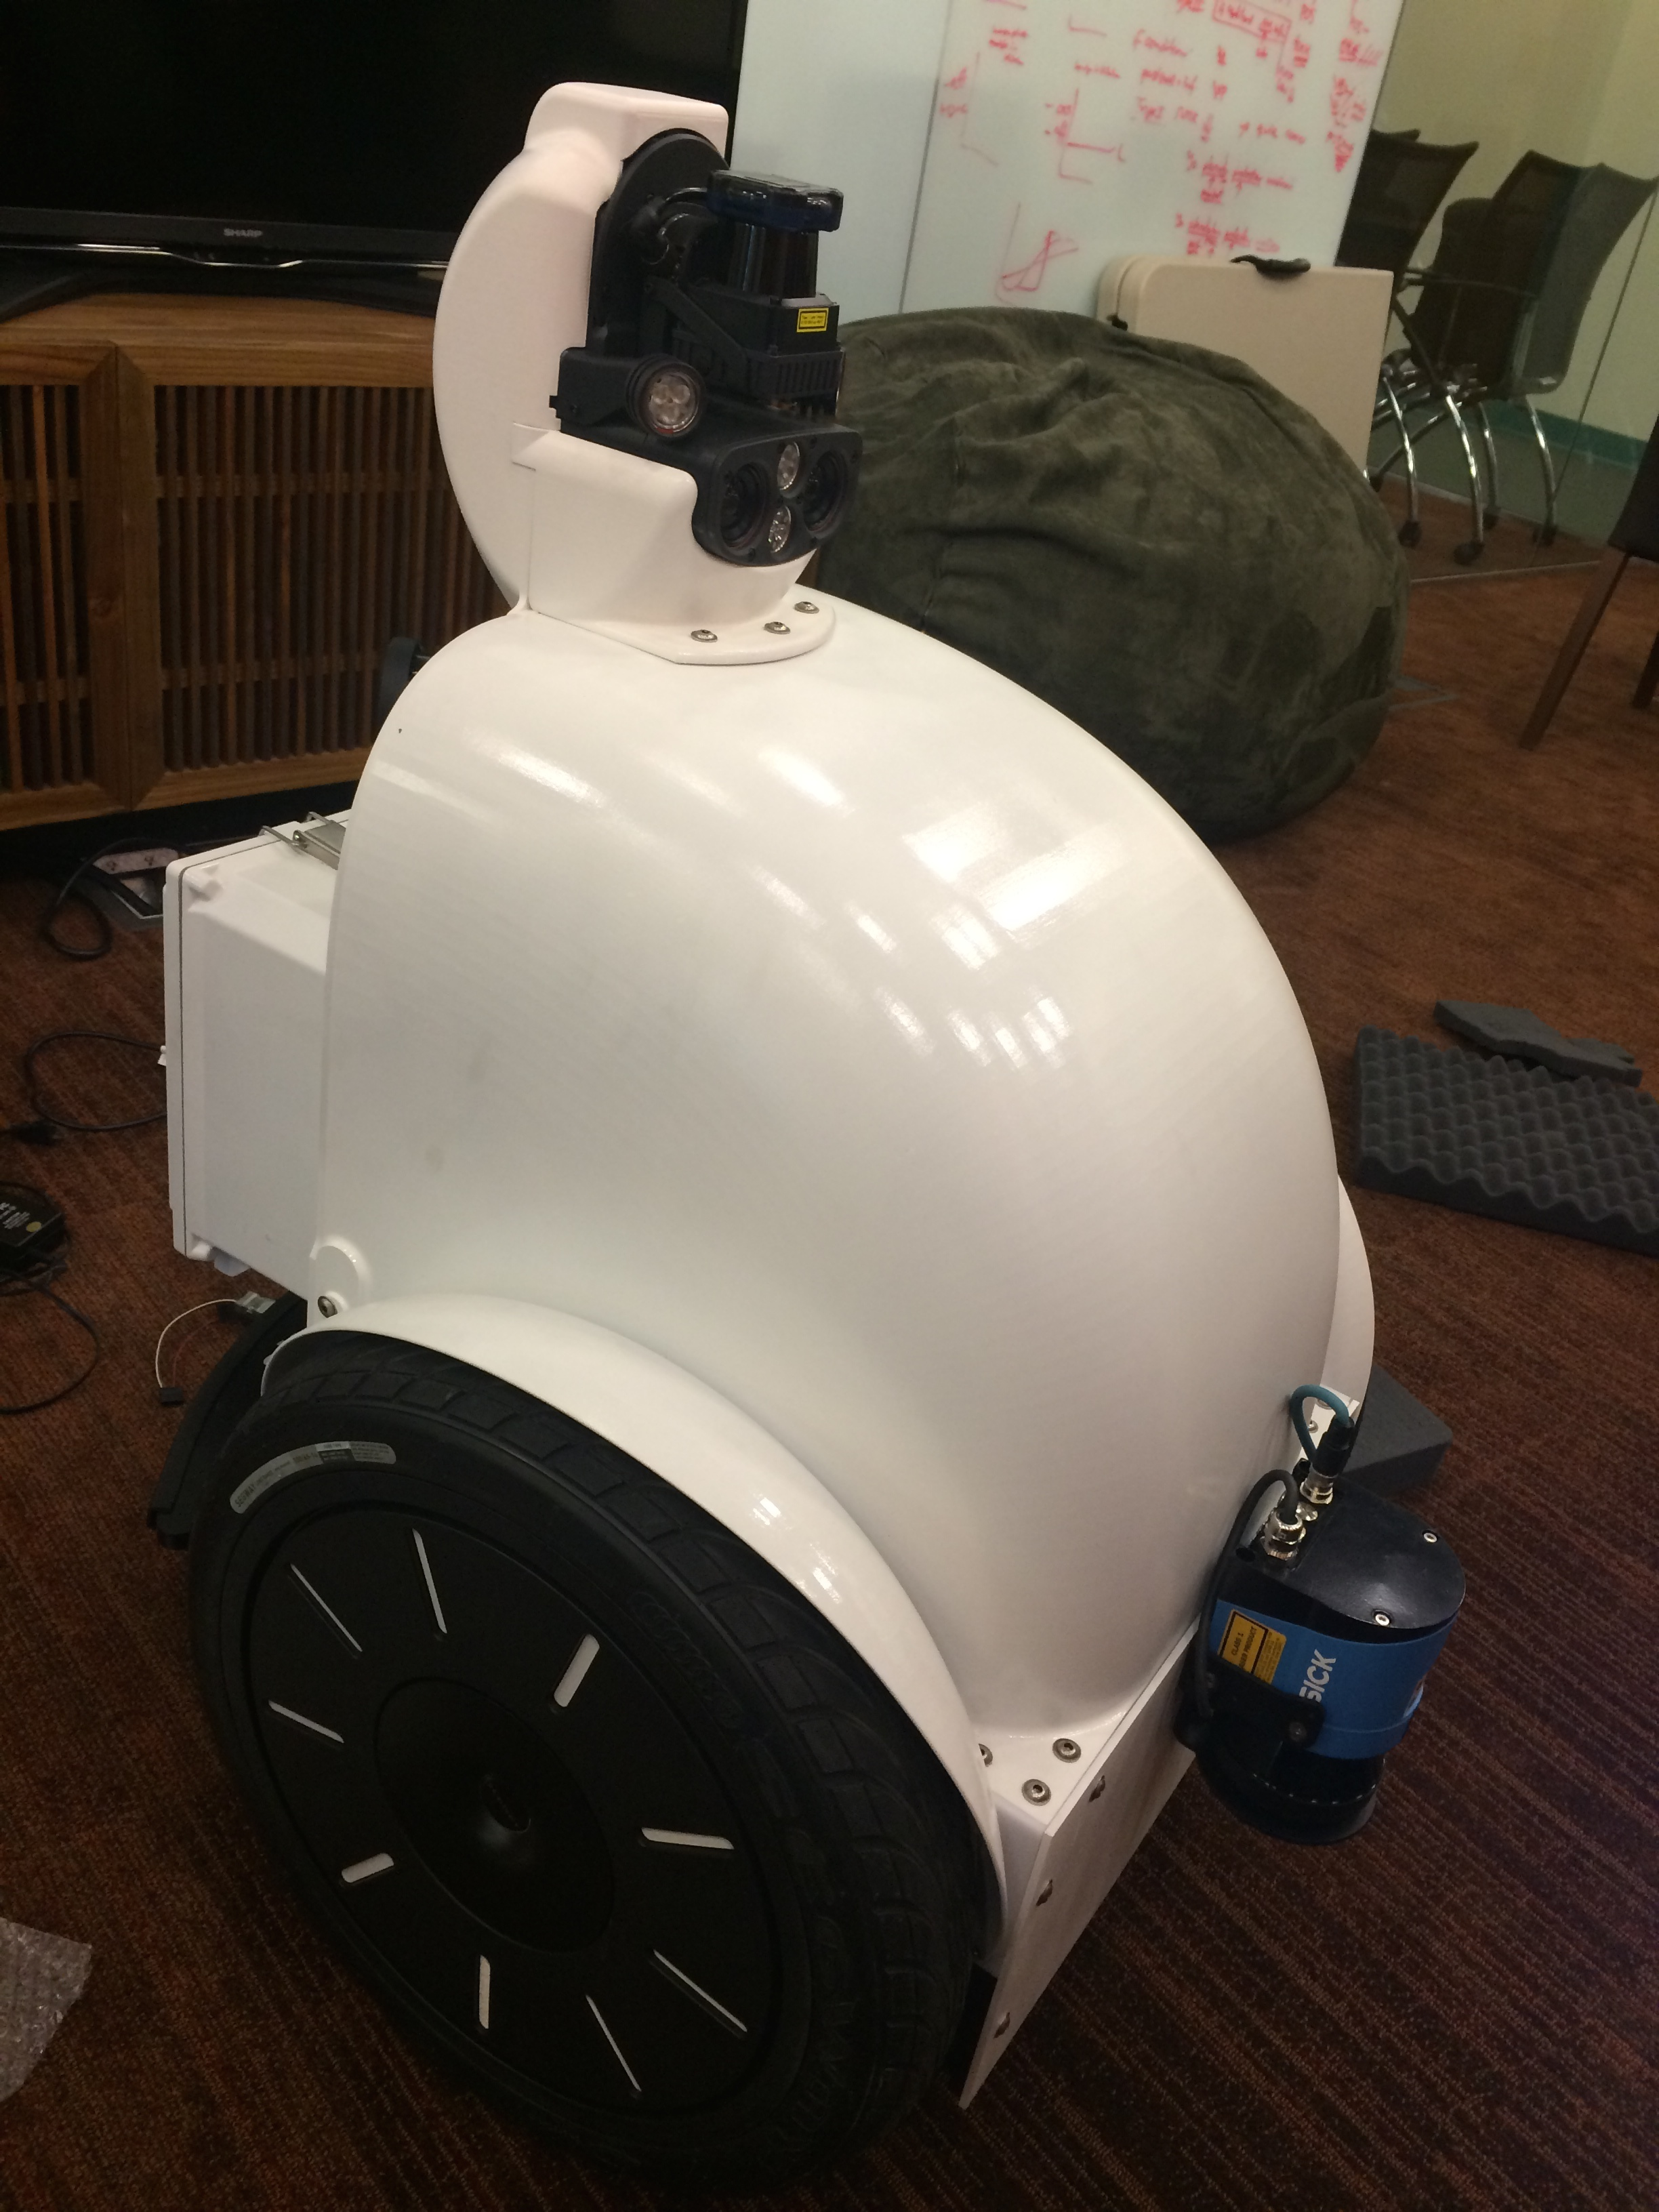
\includegraphics[scale=0.1]{pics/jackrabbot.jpeg}
\end{center}
   \caption{The Jackrabbot}
\label{fig:long}
\label{fig:onecol}
\end{figure}

\section{Technical Approach}

In order to train the Jackrabbot to navigate like a human, we will manually drive the robot through crowded environments. While driving the robot, we will record the images being captured by all of the cameras $(c_1...c_n)$ on the device as well as the manual control input to the robot. The manual control input at time t, $\theta_t$ will be recorded as the difference between the orientation at time t, $\phi_t$ and at time t-1, $\phi_{t-1}$. To make this a classification problem, $\theta_t$ will represent a bin of angles. For example, if $\phi_t$ and $\phi_{t-1}$ are measured in degrees in [-180...180], we compute $\theta$ as: 
\begin{center} 
$\theta = \lfloor((\phi_t - \phi_{t-1}) / binsize)\rfloor$
\end{center}

After driving the robot for some time, T, we will have recorded $c_{1,t}...c_{n,t}, \theta_t$ for every t in 1..T. After recording sufficient data, we will build up a dataset of inputs and outputs that the robot can use to learn to replicate and generalize the navigation patterns recorded from the human driver. Each input will be a time sequenced set of images from all of the cameras $(c_{1,t}...c_{n,t}, c_{1,t-1}...c_{n,t-1}...c_{1,t-k}...c_{n,t-k})$, and the output will be $\theta_t$.

Using this dataset, we will develop, train, and test a convolutional neural network to predict the desired orientation given a sequence of images from multiple cameras. As will be discussed in the next section, we will be using a slightly modified architecture to take these multiple images as input. We will try a different architectures and operate on different subsets of this data. For example, we can compare the effectiveness of using a single camera vs. multiple cameras or using images from varying sequence lengths (i.e. varying the value of k). How we will train these different models will be discussed more in the next section.

Finally, once we have trained and tested these models we need a good way to compare their performance. One measure will simply be the classification accuracy (the percent of the test samples for which we correctly predict $\theta$). The problem with this metric is that it does not account for the correlation between the output classes. For example while two orientations may fall in different bins, they may actually be rather close to each other. We compute an evaluation metric on the average distance in bins between the correct $\theta$ and predicted $\theta$. The final numeric metric that we will evaluate is the runtime of the network. For robotic applications, it is critical for the navigation system to work in real time.

While numeric metrics are important, it is equally critical to develop a set of qualitative metrics to debug mistakes being made by the classifier. To visualize these errors, we will create maps that compare the ground truth trajectory to the predicted trajectory. We will also visualize the weights for the first convolutional layer of the network. We can decompose the weights for our multi-image input to visualize filters that act over x, y, and t.

To evaluate the performance between different methods, we would also like to take benchmarks of the total training and test time of each method and plot them against the test accuracy.

We propose two main methods of visual processing as inputs into a linear classifier, SVM and Softmax, that will determine the direction the Jackraboot should turn at any given moment. We will also train a linear classifier, SVM and Softmax, on features obtained from computer vision techniques such as depth calculation, object detection, and motion tracking, as a baseline for the convolutional neural network based learning. After characterizing the performance of these two main methods, shallow vs. deep learning, variants of each method based on modifying the inputs and features will be explored to further optimize accuracy. Preprocessing will include zero-mean and normalization to [-1, 1]. The dataset will be randomly split into training, validation, and test sets into 70\%, 20\%, and 10\% of the collected dataset to tune the hyperparameters and test the final performance.

The stereo camera will need to be calibrated to find the fundamental matrix. Once it is found,  the following features will be extracted from the raw input image and put through an SVM and Softmax linear classifier. 

\begin{itemize}
\item HOG features
\item Depth map calculated from the stereo camera
\item Motion map with tracked motion vectors in place of each pixel within the bounding box of detected objects
\end{itemize}


\section{Progress}
Since we were not able to set up the robot until Monday, Feb 23rd, we have been focusing on setting up the framework and getting all the libraries set up. We have set up OpenCV and Caffe on farmshare and have run some tests. As for the Jackrabbot, we installed the battery and set up the virtual machine. However, the charger has not arrived yet, so we could not collect any data. In the meantime, we have implemented the preprocessing and data visualization code.

\section{Milestones Left}
\begin{itemize}
\item 2/25/15: Collect Data
\item 2/27/15: Convolutional Neural Network
\item 2/27/15: Object detection and tracking
\item 3/1/15: Learning on Vision
\item 3/8/15: Compare Numerical Results from Each Algorithm
\end{itemize}

\begin{thebibliography}{1}

\bibitem{alvinn}
Pomerleau, Dean A., "ALVINN, an autonomous land vehicle in a neural network", Carnegie Mellon University, 1989. http://repository.cmu.edu/cgi/viewcontent.cgi?article=2874\&context=compsci.

% CS231N Notes
\bibitem{andrej}
Li, Fei-Fei and Karpathy, Andrej. "CS231n: Convolutional Neural Networks for Visual Recognition", 2015. http://cs231n.github.io.

% CS231A Textbooks
\bibitem{A1}
D. A. Forsyth and J. Ponce. \emph{Computer Vision: A Modern Approach (2nd Edition)}. Prentice Hall, 2011.
\bibitem{A2}
R. Hartley and A. Zisserman. \emph{Multiple View Geometry in Computer Vision}. Cambridge University Press, 2003. http://searchworks.stanford.edu/view/5628700.
\bibitem{A3}
R. Szeliski. \emph{Computer Vision: Algorithms and Applications}. Springer, 2011. http://searchworks.stanford.edu/view/9115177.
\bibitem{A4}
D. Hoiem and S. Savarese. "Representations and Techniques for 3D Object Recognition and Scene Interpretation", \emph{Synthesis lecture on Artificial Intelligence and Machine Learning}. Morgan Claypool Publishers, 2011. http://searchworks.stanford.edu/view/9379642.
\bibitem{A5}
Gary Bradski, Adrian Kaehler. \emph{Learning OpenCV}, O'Reilly Media, 2008. http://searchworks.stanford.edu/view/7734261. 


\end{thebibliography}

\end{document}